\documentclass{vldb}

%%% Packages
\usepackage{graphicx}
\usepackage{balance}
\usepackage{tikz}
\usepackage{standalone}
\usepackage{subfigure}
\usepackage{colortbl}

%%% TikZ libraries
\usetikzlibrary{backgrounds, positioning, decorations.pathreplacing, calc, fit}
\usetikzlibrary{shapes}

%%% Macros
\newcommand{\tbr}{{\color{red}\textbf{[TO BE REVISED]}}}
\newcommand{\tbd}{{\color{red}\textbf{[TO BE DONE]}}}

\newcommand\diag[4]{%
  \multicolumn{1}{p{#2}|}{\hskip-\tabcolsep
  $\vcenter{\begin{tikzpicture}[baseline=0,anchor=south west,inner sep=#1]
  \path[use as bounding box] (0,0) rectangle (#2+2\tabcolsep,\baselineskip);
  \node[minimum width={#2+2\tabcolsep-\pgflinewidth},
        minimum  height=\baselineskip+\extrarowheight-\pgflinewidth] (box) {};
  \draw[line cap=round] (box.north west) -- (box.south east);
  \node[anchor=south west] at (box.south west) {#3};
  \node[anchor=north east] at (box.north east) {#4};
 \end{tikzpicture}}$\hskip-\tabcolsep}}

\begin{document}

% Title
\title{Building an Image Recognition System}
\subtitle{Project Report}

% Author(s)
\numberofauthors{1}

\author{
\alignauthor
	Daniel Kocher\\
  \affaddr{Department of Computer Sciences \\ University of Salzburg}\\
  \email{Daniel.Kocher@stud.sbg.ac.at}
}

\maketitle

\begin{abstract}
Automatic understanding of images (and videos) is a challenging problem in
computer vision. There exist different low- and high-level approaches to tackle
this problem.

In this paper, a project is presented which uses a higher-level approach, i.e. an
attribute database. Based upon this database, a Bag-of-Visual-Words (BoW)
representation is obtained and classifiers are trained for each attribute in the
database. The average precision of these classifiers is then evaluated for
different parameters. Furthermore, these classifiers are then used to do scene
recognition based on attribute classifiction. Again, the predictive power of this
approach is evaluated for different parameter configurations.
\end{abstract}

\section{Introduction}
\label{sec:introduction}

Representing images can be done on different levels: there exist
low-level approaches, e.g. the \emph{spatial pyramid}~\cite{Lazebnik:2006} which
take spatial information into account, and higher-level approaches, like attribute
databases.

Attribute databases represent images in terms of present or absent attributes.
Such a representation is considered \emph{interpretable} because it is intuitive
for human beings to describe an image in terms of attributes. For example,
consider an image of the Caribbean beach in the summer. Humans see the sun, the
ocean, the beach, people sunbathing, some boats and the horizon. Then, an
intuitive description of this image would be e.g. sunny, water/sea, sleeping,
crowded, boating, sandy and sky. If another human being reads such a description,
he/she will probably predict an image of a crowded beach in the summer. Hence,
the image representation through attributes is a so-called
\emph{semantic encoding} of images. Moreover, attributes are machine-detectable
which is important (otherwise it would be useless in image processing).

For this project, the SUN Attribute Database~\cite{Patterson:2012} is used, hence
we will always refer to this database when talking about attribute databases.
Using such a database, one can train a classifier for each of these attributes
which can then be used to predict attribute presence for a given, previously
unseen image. When we proceed like this, we get $n$ classsifiers if there are $n$
attributes provided by the database. Next, we can represent an image as a
$n$-dimensional vector which describes the image, again, in terms of $n$
attributes.

This enables us to extract such $n$-dimensional vectors from another set of
images. This set of images contains $m$ scenes which can be used to train another
(nearest neighbors) classifier to predict scenes based on a given $n$-dimensional
attribute vector of a previously unseen image. The used scene database was created
by Lazebnik et al.~\cite{Lazebnik:2006}.

The remainder of this paper is organized as follows.
Section~\ref{sec:general-approach} describes the general approach (the pipeline)
of the project. It also contains more detailed information about the main
concepts used in the pipeline, i.e. a description of the image databases, the
feature extraction in use, the codebook generation and the scene recognition.
Section~\ref{sec:implementation-details} summarizes some implementational
details and assumptions, Section~\ref{sec:results} shows some results of the
evaluation of this project and, finally, Section~\ref{sec:conclusion} concludes
this report.

\section{General approach}
\label{sec:general-approach}

This sections summarizes the main steps involved in this project. This includes
a description of the used image databases, an illustration of the computation
pipeline and more detailed descriptions for the most important parts of this
pipeline.

\tbr

\subsection{Image Databases}
\label{subsec:image-databases}

\paragraph*{Attribute Database}
\label{par:attribute-database}

As mentioned before, we utilize the SUN Attribute Database~\cite{Patterson:2012}
to train classifiers for each of the 102 attributes. This database provides
14,340 images and 102 attributes for each image. For each such image, 3 persons
(\emph{voters}) voted for attributes to be present or not. An attribute is
considered present if at least 2 out of the 3 voters voted for the attribute to
be present. Otherwise the attribute is considered absent. To be able to evaluate
the accuracy of the classifiers in a robust manner, multiple classifiers for the
same attributes are trained and their average prediction accuracy is evaluated.
The splits used in the original paper are available online. However, for the
purpose of this project splits are generated on-the-fly.

\paragraph*{Scene Database}
\label{par:scene-database}

For the scene recognition evaluation, we use the 15 scenes dataset of Lazebnik
et al.~\cite{Lazebnik:2006}. This dataset contains 4485 images and 15 categories.
Again, splits into training and test data are generated on-the-fly using random
selection of images for each of the scene categories

See Section~\ref{subsec:high-level-pipeline} for details on how the splits of
both databases are generated.

\tbr

\subsection{High-Level Pipeline}
\label{subsec:high-level-pipeline}

The high-level pipeline consists of 5 parts: Adjusting the settings if necessary,
generating a scaler and a clustering, generating the codebook/bag-of-visual-words
representation and training the classifiers, recognizing scenes based upon the
trained classifiers and obtaining the results. Obviously, the 3 parts in the
middle are the most important parts. In the following, we will discuss these three
parts in more details. Figure~\ref{fig:high-level-pipeline} shows an illustration
of the pipeline.

\begin{figure}
  \centering
  \begin{tikzpicture}
    \def\minwidth{\widthof{GENERATE SCALER/CLUSTERING} + 50pt}
    \def\minheight{\heightof{GENERATE SCALER/CLUSTERING} + 10pt}
    \node[draw, rectangle, thick, minimum width = \minwidth,
      minimum height = \minheight] at (0, 0) (settings) {\bfseries SETTINGS};
    \node[draw, rectangle, thick, minimum width = \minwidth,
      minimum height = \minheight, below = 0.5 of settings] (scaler-clustering)
      {\bfseries GENERATE SCALER/CLUSTERING};
    \node[draw, rectangle, thick, minimum width = \minwidth,
      minimum height = \minheight, below = 0.5 of scaler-clustering]
      (bow) {\bfseries GENERATE CODEBOOK/BOW};
    \node[draw, rectangle, thick, minimum width = \minwidth,
      minimum height = \minheight, below = 0.5 of bow] (scene-recognition)
      {\bfseries RECOGNIZE SCENES};
    \node[draw, rectangle, thick, minimum width = \minwidth,
      minimum height = \minheight, below = 0.5 of scene-recognition] (results)
      {\bfseries RESULTS};


    \draw[->, >=stealth] (settings.south) -- (scaler-clustering.north);
    \draw[->, >=stealth] (scaler-clustering.south) -- (bow.north);
    \draw[->, >=stealth] (bow.south) -- (scene-recognition.north);
    \draw[->, >=stealth] (scene-recognition.south) -- (results.north);
  \end{tikzpicture}
  \caption{High-level pipeline}
  \label{fig:high-level-pipeline}
\end{figure}

The SETTINGS step is just a configuration step, where  parameters like
the number of classes for the clustering or the number of training/test images per
split can be configured.

The second stage is quite obvious. First of all we need a consistent scaling of
feature vectors throughout the pipeline. In the following, all feature vectors
are considered scaled, even without explicitly stating it. Furthermore, we need
a clustering mechanism which is used in the codebook generation. In this project,
a simple $k$-means++ clustering is used. Of course, one could just replace both,
the scaler and the clustering, by different/more advanced approaches.

In the third stage, the codebook/bag-of-visual-words representation is obtained.
This includes multiple steps, which are: 
\begin{enumerate}
  \item For each attribute multiple training/test splits are generated on-the-fly
  \item For each image of a split, feature vectors are obtained
  \item These feature vectors are predicted using the previously generated
    $k$-means++ clustering
  \item Generate histograms for each predicted feature vector
  \item Using the histograms of training data, a classifier is trained for each
    attribute
  \item Using the histograms of test data, the classifier is evaluated for each
    attribute (mean precision and standard deviation over all splits for an
    attribute)
  \item Classifiers are stored on the filesystem (to be used in the scene
    recognition stage)
\end{enumerate}

Next up is the scene recognition stage which is also divided into multiple steps:
\begin{enumerate}
  \item The image of each scene is divided into training and test images
  \item Extract the feature vector for each training image (this feature vector
    has to be consistent with the feature vector used in the previous stage)
  \item Generate histograms for each feature vector 
  \item Use histograms as input for the classifiers to create an $n$-dimensional
    vector for each training image ($n$ is the number of classifiers/attributes)
  \item Train a $k$-nearest neighbor classifier using these $n$-dimensional
    vectors and the corresponding scene name
  \item Use $k$-nearest neighbor classifier to predict the test images (more
    precisely, their $n$-dimensional vectors)
\end{enumerate}

The last stage is the evaluation of the results.

\tbr

\subsection{Scaler}
\label{subsec:scaler}

For the purpose of classification it is desirable to scale feature vectors. In
our case, a scaler is created which is then used to project every value of the
feature vectors to range $(0, 1)$. This scaler has to be created before doing any
feature extraction (more precisely before any of the feature vectors is actually
used). This is important because we need to use the same scaling for all steps
involving feature vectors, namely the clustering, the codebook generation
and the scene recognition.

\tbr

\subsection{Clustering}
\label{subsec:clustering}

In order to do a codebook generation, we need a clustering mechanism. For this
purpose we use $k$-means++ clustering, which is similar to the well-known
$k$-means clustering but does not just pick random elements to start with.
Given a set of feature vectors, the $k$-means++ algorithm generates $k$ clusters
during the training phase. In the prediction phase, it predicts the cluster for
a given, potentially unknown feature vector. In this project, 512 clusters were
used (this is adjustable in the first stage of
Figure~\ref{fig:high-level-pipeline}).

\tbr

\subsection{Feature Extraction}
\label{subsec:feature-extraction}

\emph{Dense Scale-Invariant Feature Transform} (Dense SIFT) is used to extract
feature from images. Before extracting the actual feature, every image is scaled
to the same size, namely $256\times256$, and converted to grayscale.
\emph{Dense} SIFT, because we do not just let the SIFT algorithm detect keypoints
but instead use a dense grid. This grid has a step size of $16$ between two
keypoints (horizontally and vertically). For $256\times256$ pixels this results
in a total number of $256$ keypoints ($16\times16$). Then, for each such keypoint,
the SIFT algorithm is applied. This results in a total number of $256$
$128$-dimensional feature vectors for each image.
Figure~\ref{fig:dense-sift-example} shows an example image which all keypoints
marked by a circle.

\begin{figure}
  \centering
  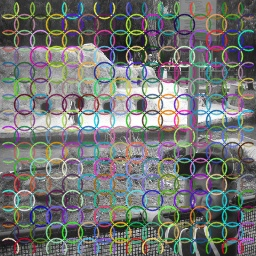
\includegraphics[width = .25\textwidth]{figs/dense_sift.jpg}
  \caption{Dense SIFT example}
  \label{fig:dense-sift-example}
\end{figure}

This method of feature extraction is used throughout the pipeline. It could also
be replaced by more advanced feature extraction techniques (e.g. taking color
information into account). This will probably lead to better overall results.

\tbr

\subsection{Bag-of-Visual-Words}
\label{subsec:bovw}

To generate a codebook the feature extraction and the clustering, described in
Section~\ref{subsec:feature-extraction} and~\ref{subsec:clustering}, respectively,
are used.
But first of all, we split the images of the SUN Attributes Database into 10
training/test splits for each attribute. In the evaluation stage, the average
precision and the standard deviation for all 10 splits are evaluated for each
attribute. Because of the sparseness of some attributes, we have two different
split modes, namely \emph{asymmetric} and \emph{symmetric}. The splits provided
online by Patterson et al.~\cite{Patterson:2012} also have these two modes.
We also use the same amounts of images as done by Patterson et al.:
\begin{description}
  \item[asymmetric] 300 training images (150 positive and 150 negative samples),
    100 test images (150 positive and 150 negative samples)
  \item[symmetric] 525 training images (25 positive and 500 negative samples),
    525 test images (25 positive and 500 negative samples)
\end{description}

For each image in a both sets (training and test), the respective SIFT feature
vector is computed. Then, the $k$-means++ clustering is used to assign each SIFT
descriptor of the feature vector (namely 256) to one of the $k$ clusters (here
$k=512$). Afterwards, a histogram with $k$ bins is generated. Each bin represents
a cluster and the previously assigned clusters are counted (height of a bin).

The histograms of all training images are then used to train a classifier for each
attribute (in total we get 10 classifiers per attribute because we have 10
different splits for each attribute). Hence, in the asymmetric mode, where only
87 attribute are evaluated (due to sparseness of attributes), we get 870
classifiers in total. In the symmetric case, we get 1020 different classifiers.
These classifiers are stored to use them again later on.

Now, it is about time to evaluate the precision of the trained classifiers.
Therefore we just use use the histograms of the test images as input for the
classifier's predict function. The classifier returns 0 for \emph{attribute is
not present} or 1 for \emph{attribute is present}. These results are compared
against the reference results and the total precision is stored for each
classifier instance. To conclude this stage, the average precision and the
standard deviation are computed over all 10 instances of an attribute classifier.

\tbr

\subsection{Scene Recognition}
\label{subsec:scene-recognition}

This is the final computational stage (the results stage is just a presentation
layer). In this stage, we also generate splits but this time splits for each of
the 15 scenes. For each scene we use 80\% of the images as training data and the
remaining 20\% as test data. This results in about 80\% training data and about
20\% test data over all scenes.

After the splits are generated, the classifiers are utilized to predict attributes
for a given image. For each image in the training data, we execute the predict
operation of all 87/102 classifiers (depending on the mode used in the codebook
generation). Concatenating all 87/102 predictions, we obtain a 87-/102-dimensional
vector for each training image.

In the next step, we train a $k$-nearest neighbor classifier using all
87-/102-dimensional vectors of the training data and their corresponding scene
labels. In this project, we use $k = 3$ for the nearest neighbor classification.

The nearest neighbor classifier is used to categorize given images represented
as 87-/102-dimensional vectors. Therefore, we also predict the 87/102 attributes
of the images in the test dataset to obtain 87-/102-dimensional vectors for
these images. In the last step, we just used the $k$-nearest neighbor classifier
to predict the scene of each test image.

\tbr

\section{Implementation Details}
\label{sec:implementation-details}

This section contains some details about the actual implementation.

The whole project is implemented in Python 2.7.6. Feature extraction and image
processing in general is done using OpenCV 3.1 and scikit learn is used
for classifiers, scaler and clustering.

The implementation of the split generation in the codebook generation stage always
makes sure that
\begin{enumerate}
  \item negative/positive training/test sets do not contain any duplicates (even
    though for the negative sample this is kind of unnecessary because usually
    there are at least about 13,000 images to choose from)
  \item training and test sets are disjoint
\end{enumerate}

Using the newest stable release of OpenCV 3.1 caused an inconvenience concerning
the \emph{Dense} SIFT feature extraction because in this version, Dense is not
longer supported (as it was in version 2.x). Therefore an own grid had to generate
in order to be able to use Dense SIFT (and not just SIFT).

The scaler in use is a \texttt{MinMaxScaler} and the classifiers in the codebook
generation are \texttt{LinearSVC} instances. For the $k$-means clustering, also
the corresponding scikit learn class is used. Notice that only a random sample
of the whole database is used to train the scaler and the $k$-means clustering.
To be precise, approximately 10 Dense SIFT descriptors per image are used for this
purpose.

To execute the project, one may need to adjust the settings (in
\texttt{settings/settings.py}). Here all required paths, files and parameters
can be configured.

\tbr

\section{Results}
\label{sec:results}

In this section, the experiments are discussed and some results are presented.

\begin{figure*}[ht]
  \centering
  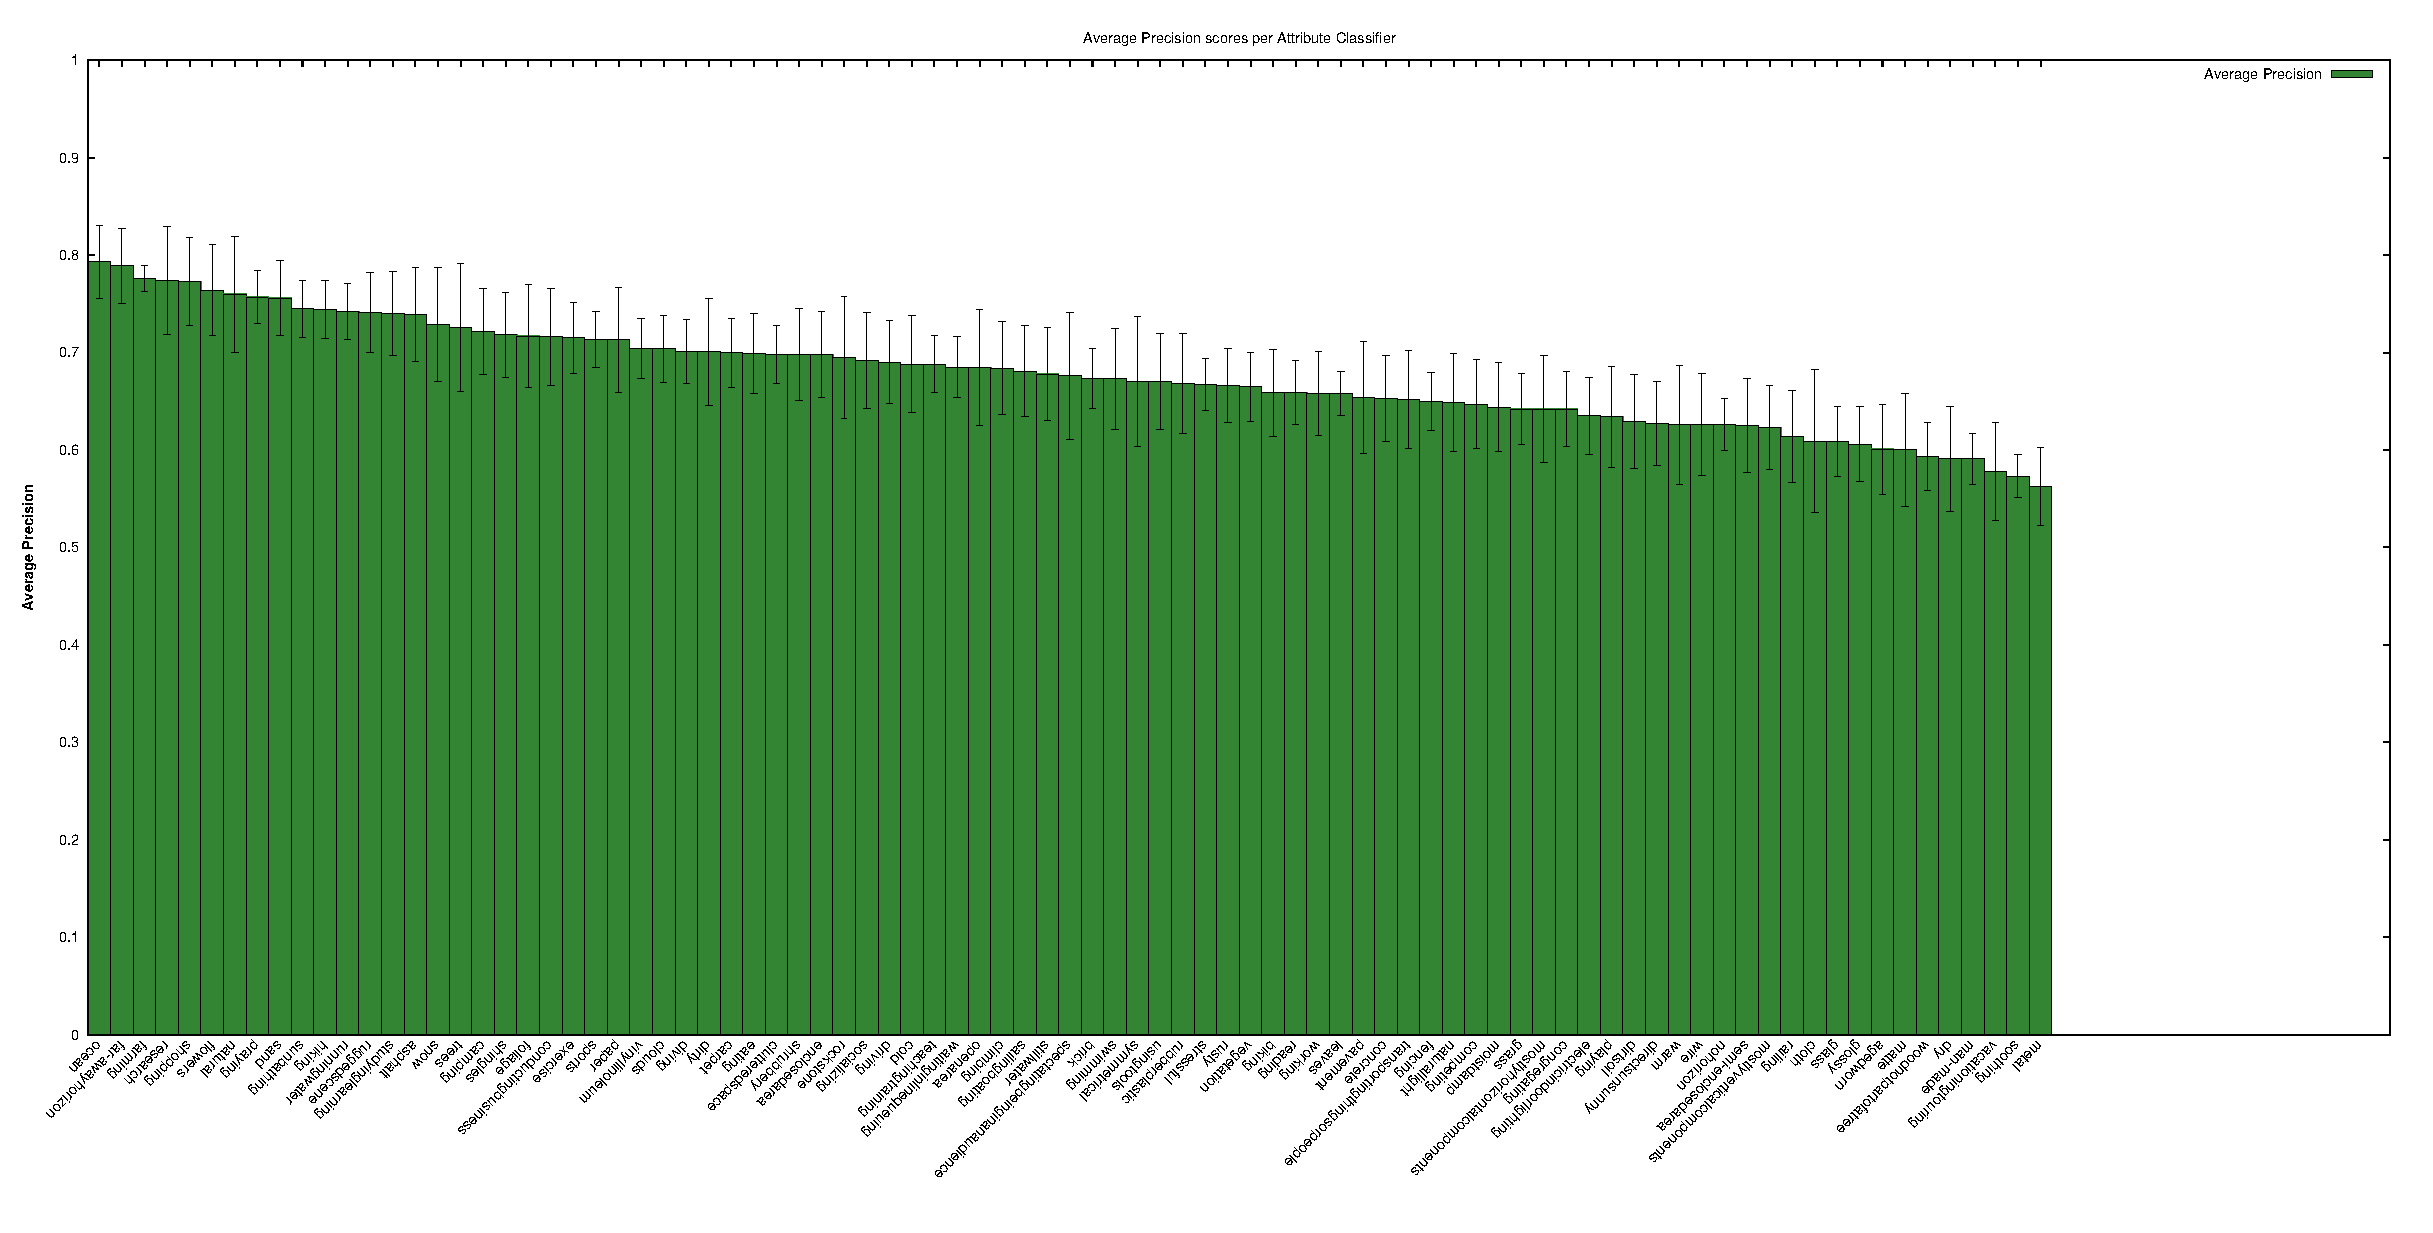
\includegraphics[width = \textwidth]{figs/scores_asymmetric_512classes.eps}
  \caption{Average scores and standard deviation of attribute classifiers
    (asymmetric splits, $k = 512$ clusters)
  }
  \label{fig:scores-classifiers-asymmetric-512}
\end{figure*}

\begin{figure}[ht]
  \centering
  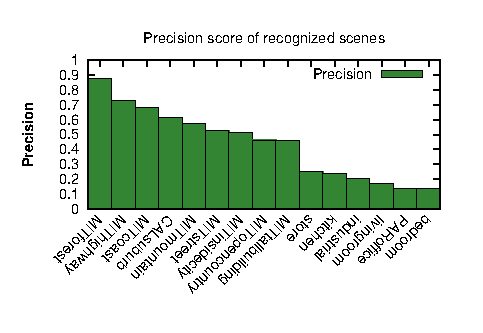
\includegraphics[width = .45\textwidth]{figs/scores_sr_asymmetric_512classes.eps}
  \caption{Scores for scene recognition \newline (asymmetric splits, $k=512$ clusters)}
  \label{fig:scores-scene-rec-asymmetric-512}
\end{figure}

In the first experiment, the asymmetric mode was used. This means the training
data contains 150 negative samples and 150 positive samples, and the test data
contains 50 negative samples and 50 positive samples. Furthermore, $k$ was set
to $512$ for the $k$-means clustering.

The first result, shown in Figure~\ref{fig:scores-classifiers-asymmetric-512},
is the average precision (and standard deviation) of each attribute classifier.
As we can see, the average precision never drops below about $55$\% and peaks
for the attributes \emph{ocean} and \emph{far-away/horizon} with about $79$\%.
Hence, even though we just used a linear support vector machine, the
classification performs well for most of the attributes.

Figure~\ref{fig:scores-scene-rec-asymmetric-512} shows the final results of the
scene catogorization. It performs well for the \emph{MITforest} scenes,
almost reaching $90$\% of correctly categorized images. However, we can also see
that this approach performs bad for some scenes, e.g. \emph{PARoffice} and
\emph{bedroom}, where the precision drops below $20$\%.

\tbr

\section{Conclusion}
\label{sec:conclusion}

In this study, the building blocks of a basic image recognition system were
discussed. The codebook generation based upon Dense SIFT feature vectors, linear
support vector machines and $k$-means clustering was described. Furthermore, all
necessary steps to implement a scene recognition based on predicted attribute
vectors and a $k$-nearest neighbor classifier were specified. We presented some
details about the actual implementation of the system described as well as the
results of this project.

\tbr

%\clearpage
% balance columns on last page
\balance

\bibliographystyle{abbrv}
\bibliography{report}

\end{document}
